% ============================================================
% IV. THỰC NGHIỆM
% ============================================================
\section{Thực nghiệm}

\begin{frame}{IV-A. Thiết lập huấn luyện}
  \begin{itemize}
    \item Tập test: 2.135 ảnh --- giữ nguyên để đánh giá cuối cùng
    \item Từ tập train gốc của FoodSeg103: chia train/val theo tỉ lệ 90/10
    \item Ba vai trò tách biệt: \texttt{train} (tối ưu) $|$ \texttt{val} (theo dõi hội tụ) $|$ \texttt{test} (đánh giá độc lập)
  \end{itemize}
  \vspace{0.5em}
  \begin{block}{Dữ liệu huấn luyện baseline: \texttt{FoodSeg103} nguyên thủy}
    Baseline giữ nguyên không gian nhãn 103 lớp, không áp dụng gộp lớp trong thiết lập chính.
  \end{block}
\end{frame}

\begin{frame}{IV-B. Kết quả}
  \begin{columns}
    \column{0.5\textwidth}
      \begin{figure}
        \centering
        
\includegraphics[width=\linewidth]{img/report/outputs/loss_curve.png}
        \caption{Train \& Validation loss}
      \end{figure}
    \column{0.5\textwidth}
      \begin{figure}
        \centering
        
\includegraphics[width=\linewidth]{img/report/outputs/metrics_curve.png}
        \caption{mIoU, mAcc, aAcc trên val}
      \end{figure}
  \end{columns}
  \begin{center}
    \begin{tabular}{ccc}
      \toprule
      \textbf{mIoU} & \textbf{mAcc} & \textbf{aAcc} \\
      \midrule
      0.31 & 0.41 & 0.79 \\
      \bottomrule
    \end{tabular}
  \end{center}
\end{frame}

\begin{frame}{IV-B. Mẫu dự đoán}
  \begin{columns}
    \column{0.55\textwidth}
      \begin{figure}
        \centering
        \includegraphics[width=\linewidth]{img/report/analyze/eval-model/07_best_cases.png}
        \caption{Các trường hợp dự đoán tốt nhất}
      \end{figure}
    \column{0.42\textwidth}
      \begin{figure}
        \centering
        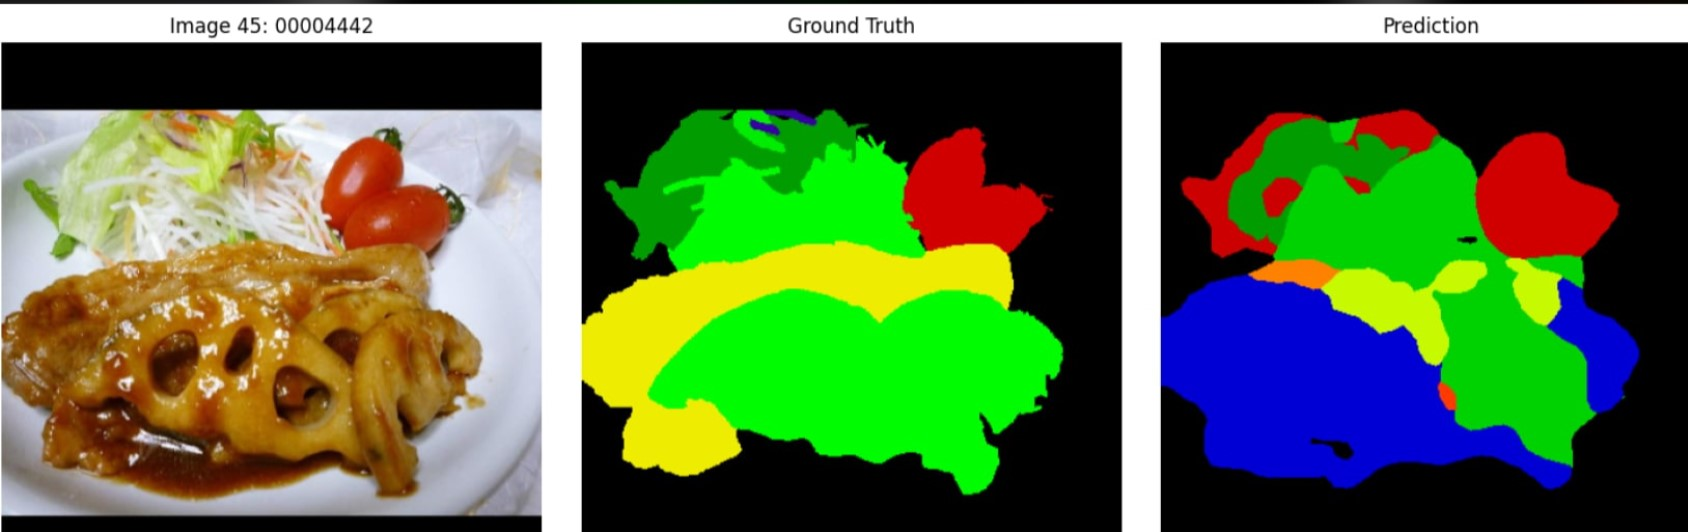
\includegraphics[width=\linewidth]{img/report/outputs/predict-problem.jpg}
        \caption{Lỗi điển hình: ranh giới mờ, chồng lấp mạnh}
      \end{figure}
      \small aAcc cao (0.79) nhưng mIoU thấp (0.31) $\to$ mô hình tốt ở vùng lớn, yếu ở vùng nhỏ và biên
  \end{columns}
\end{frame}

\begin{frame}{IV-C. Phân tích lỗi --- Pixel Acc vs.\ mIoU}
  \begin{columns}
    \column{0.5\textwidth}
      \begin{figure}
        \centering
        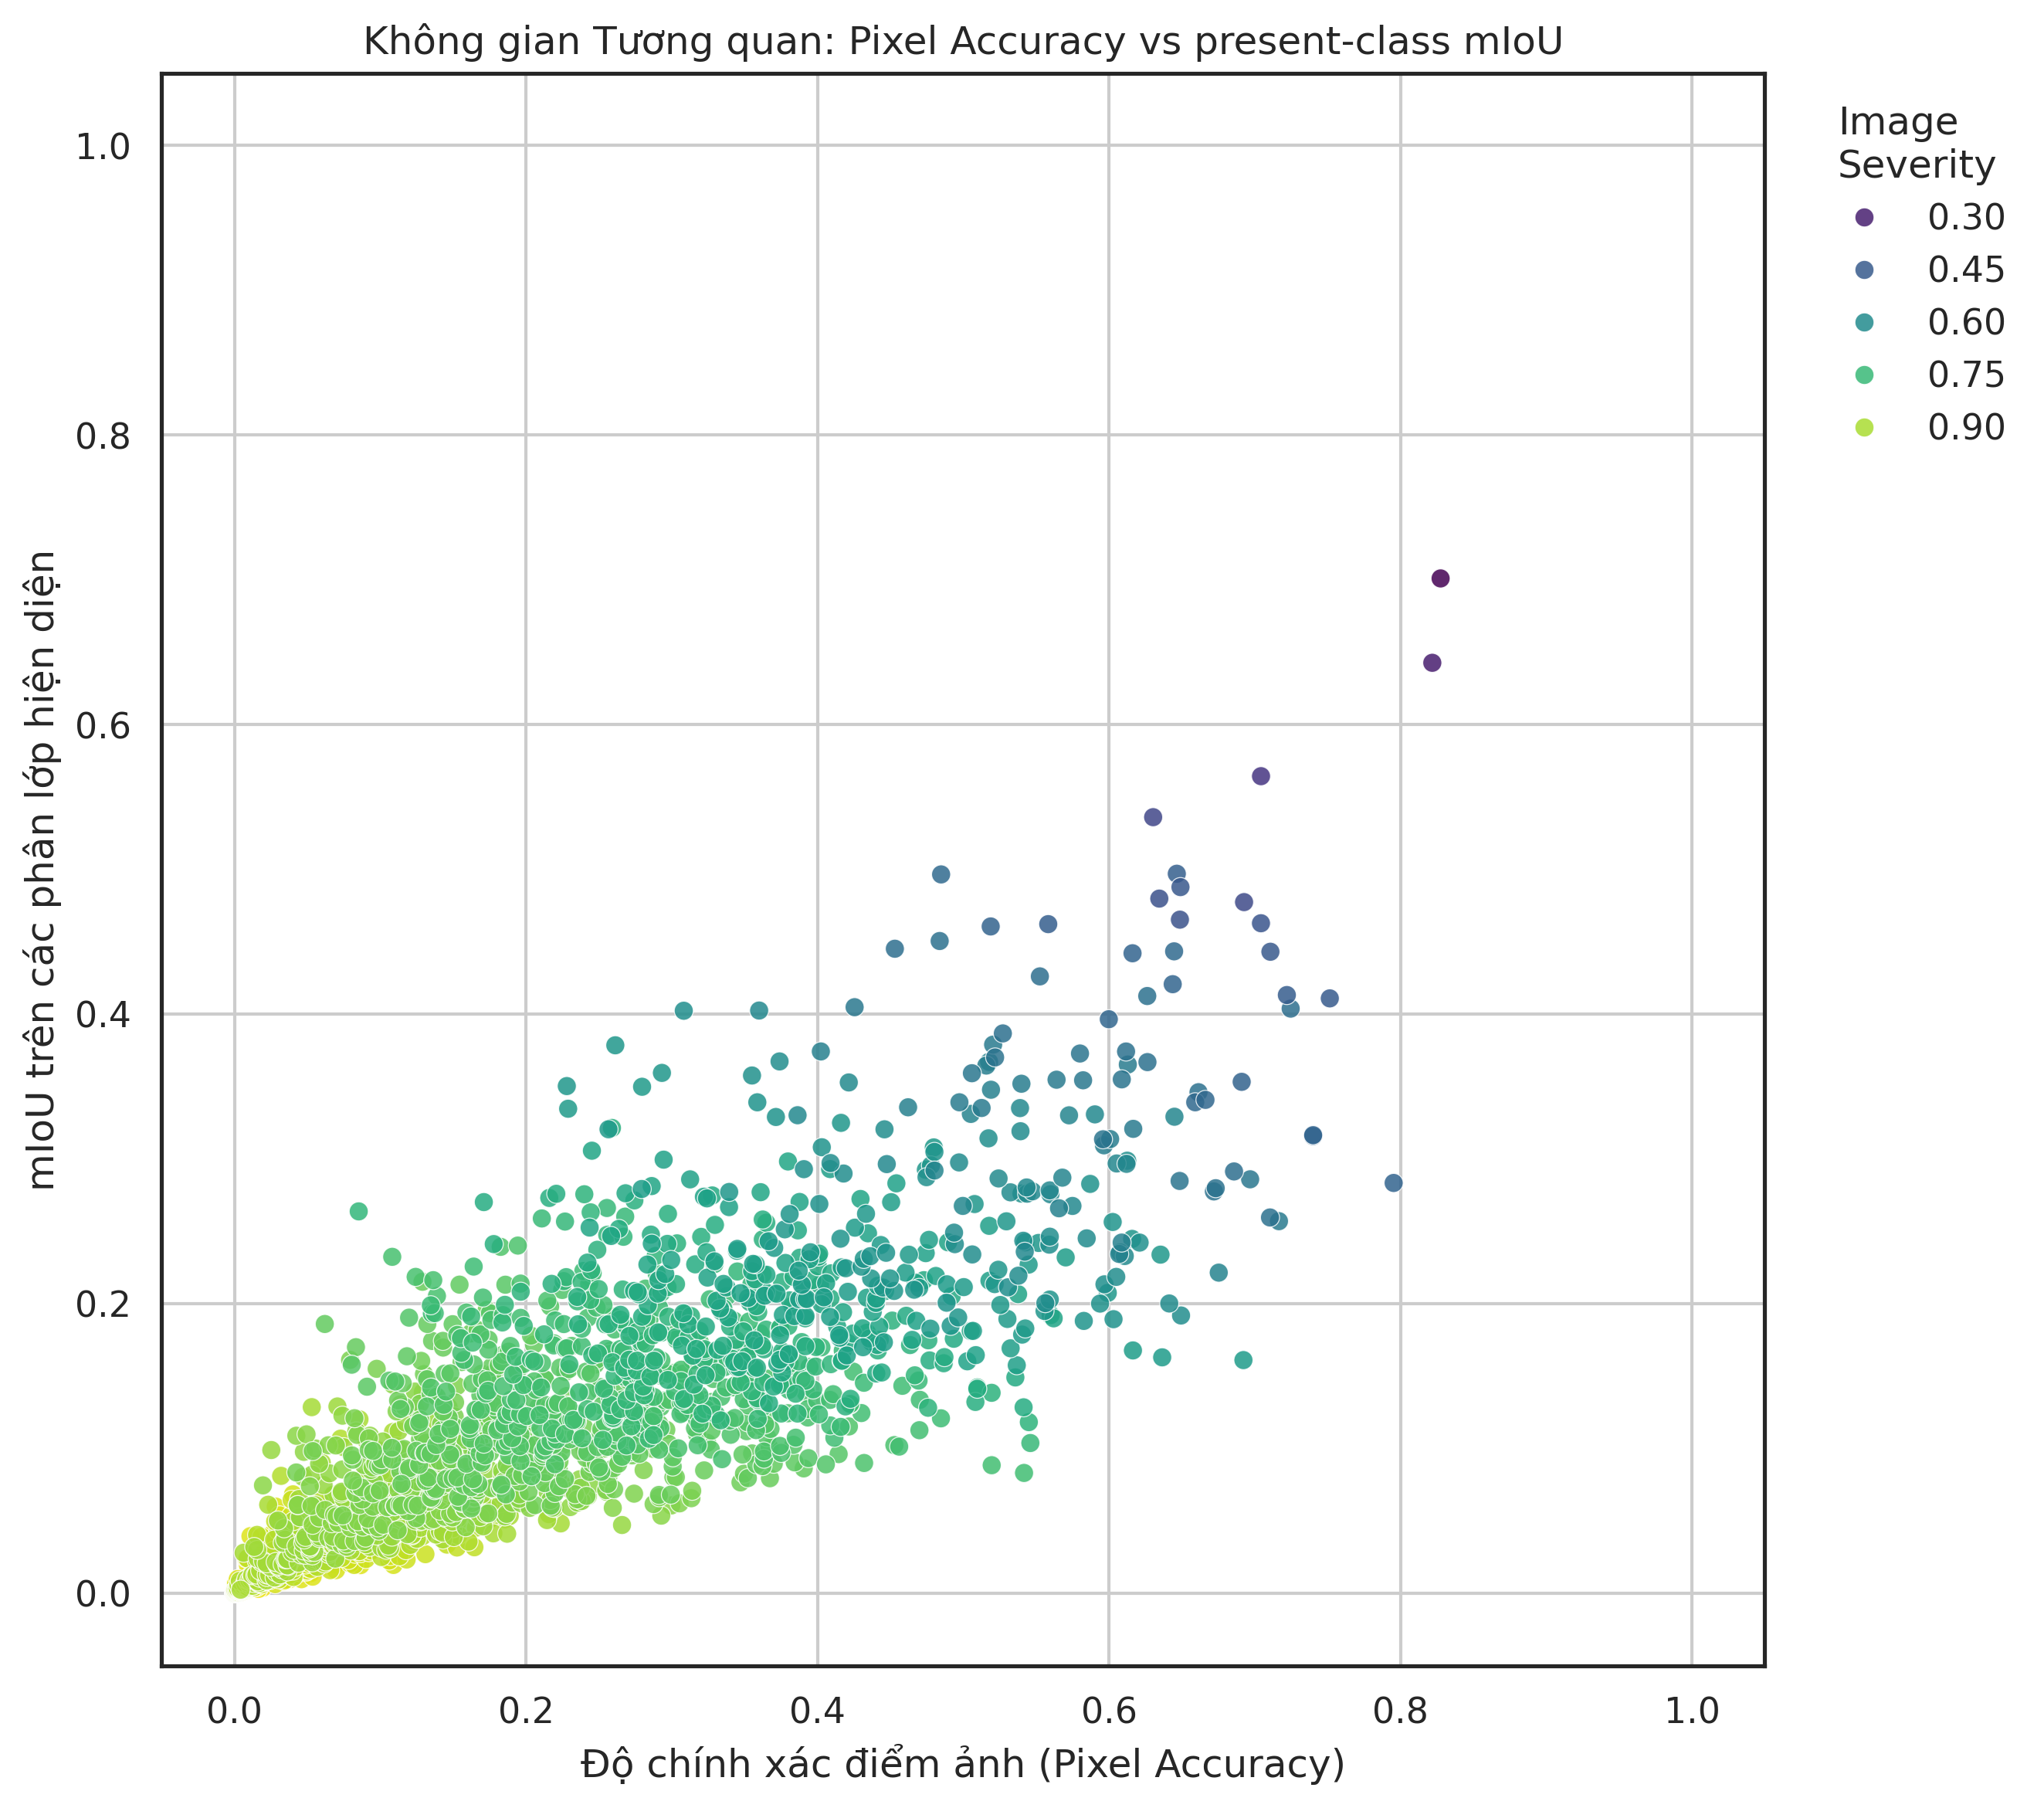
\includegraphics[width=\linewidth]{img/report/analyze/eval-model/03_pixel_acc_vs_present_miou_improved.png}
        \caption{Pixel accuracy và present-class mIoU}
      \end{figure}
    \column{0.47\textwidth}
      \begin{itemize}
        \item Pixel acc $0.3$--$0.6$ nhưng mIoU vẫn $<0.3$
        \item Pixel acc không nhạy với lỗi lớp nhỏ và vùng biên
        \item mIoU phạt đồng thời $FP$ và $FN$
        \item Điểm yếu: \textbf{định vị} sai vùng nguyên liệu, không chỉ nhận diện sai lớp
      \end{itemize}
  \end{columns}
\end{frame}

\begin{frame}{IV-C. Phân tích lỗi --- Sink class \& Confusion Matrix}
  \begin{columns}
    \column{0.5\textwidth}
      \begin{figure}
        \centering
        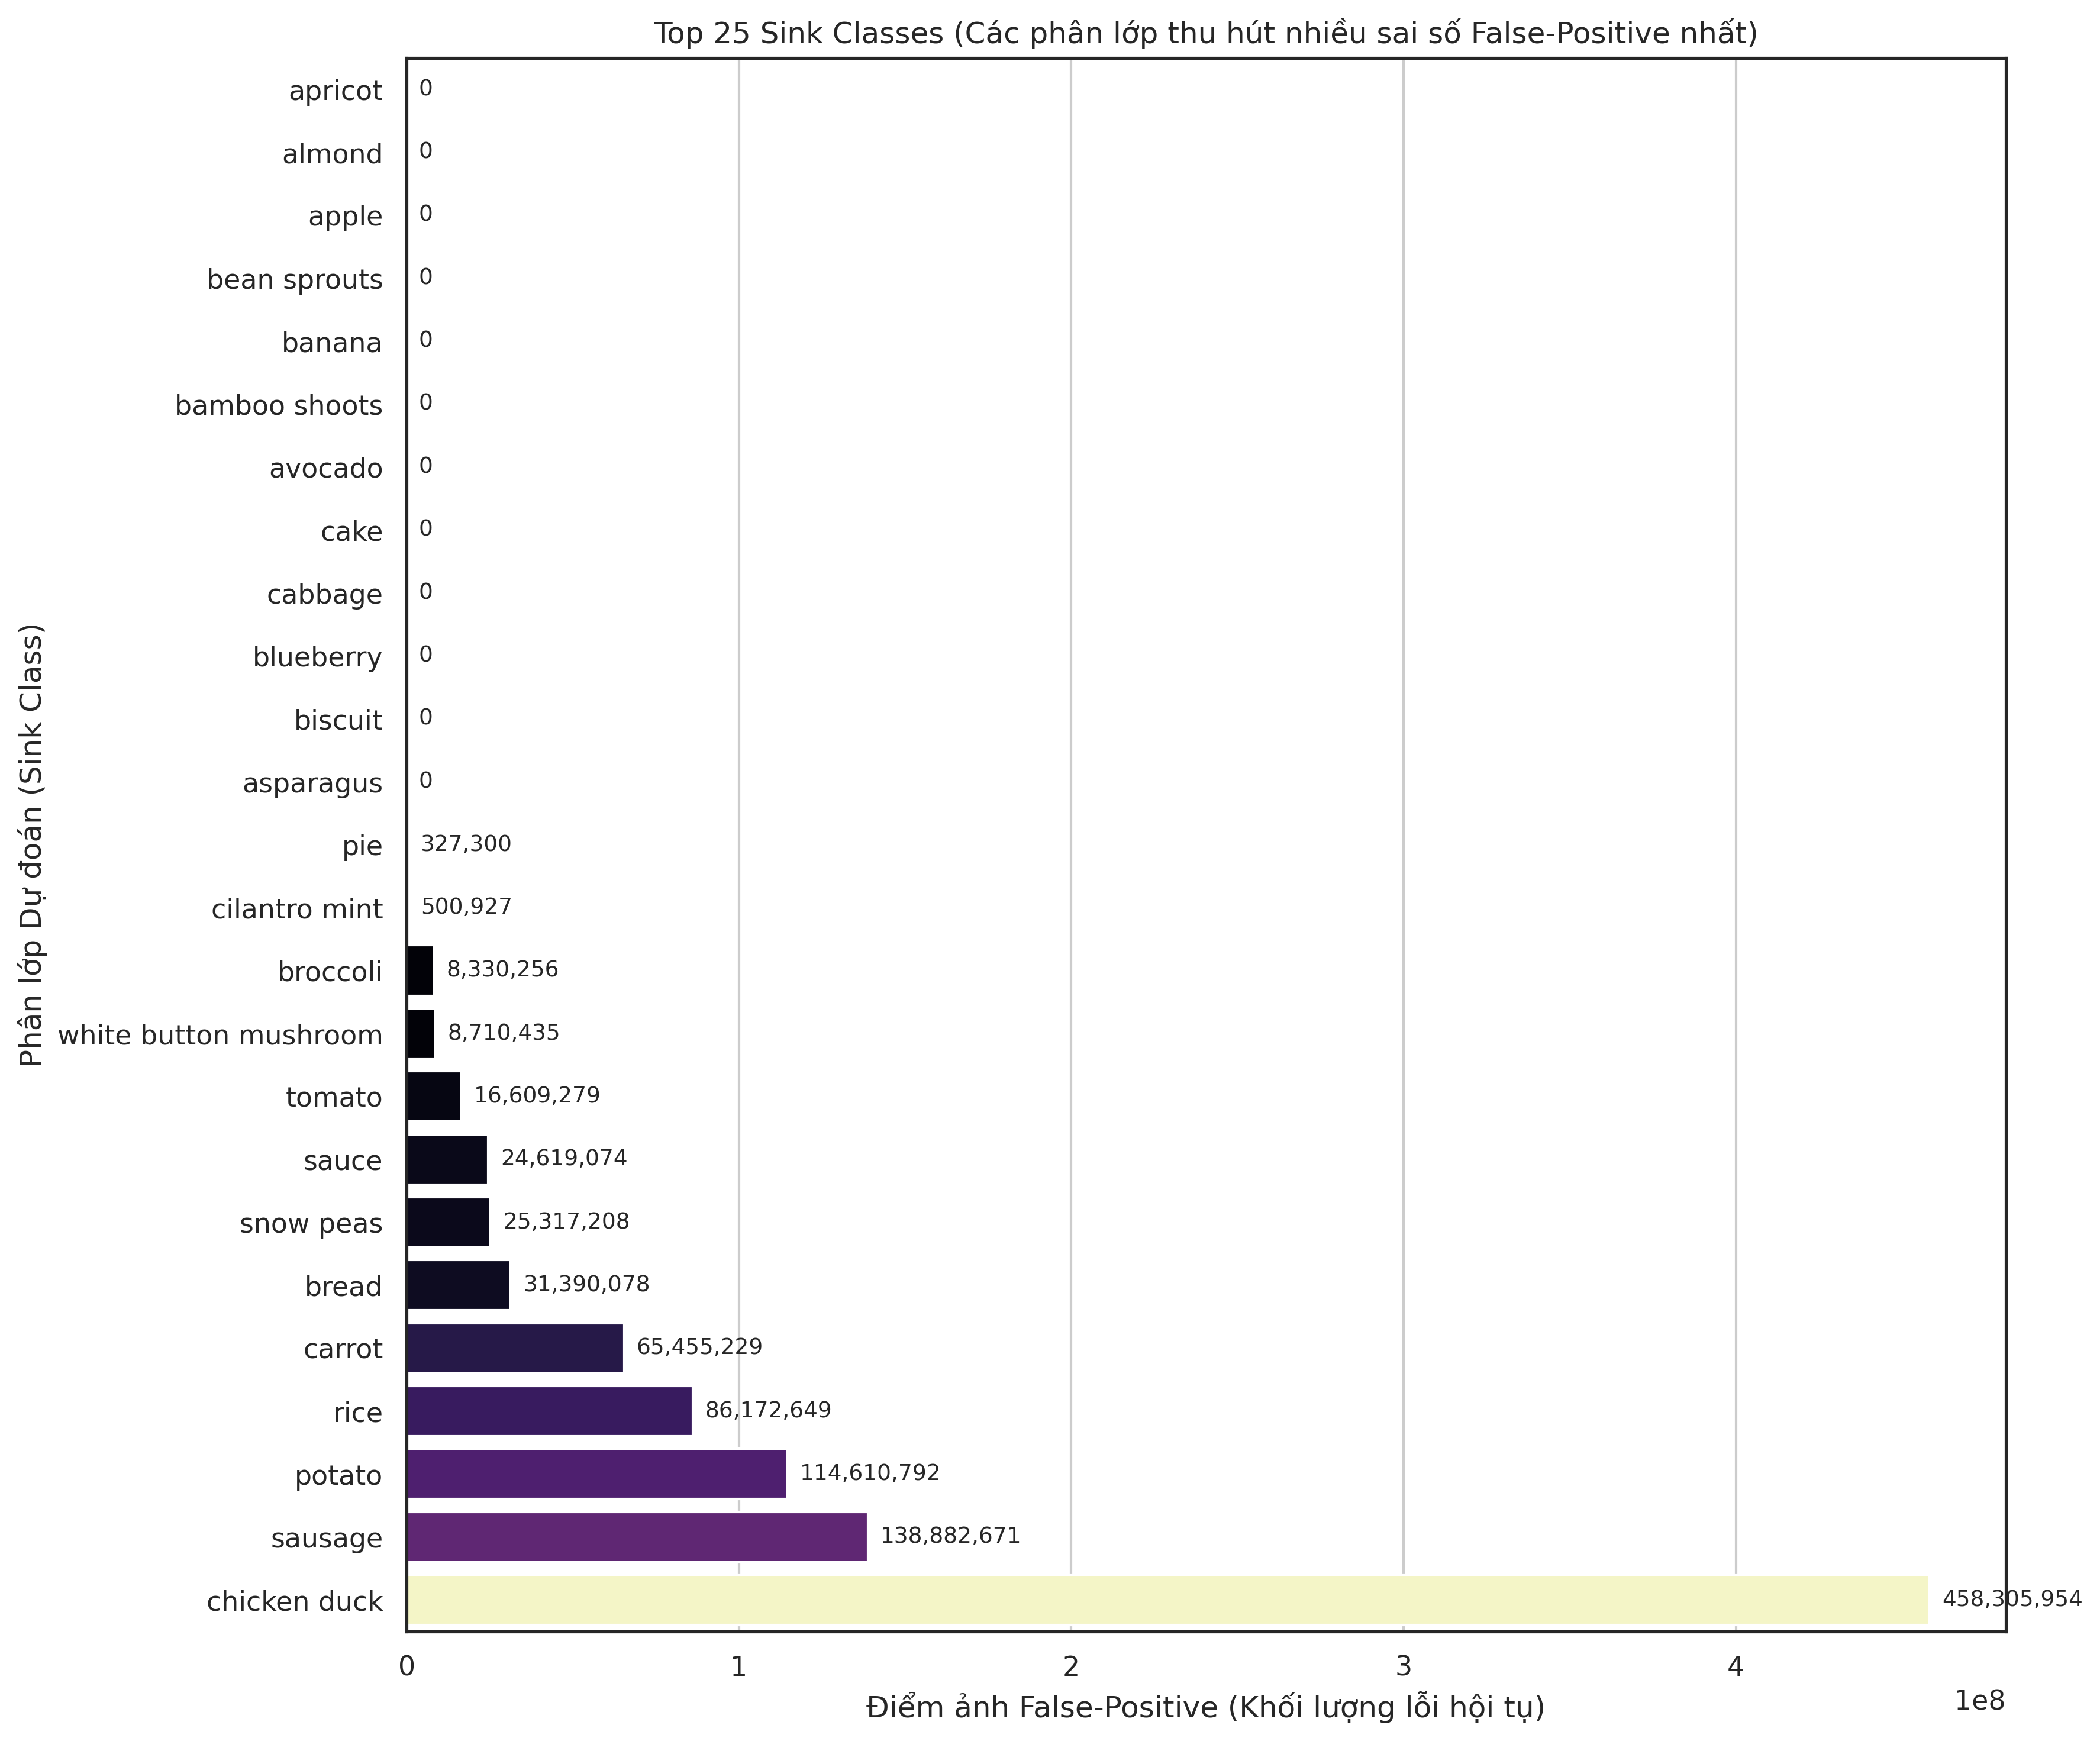
\includegraphics[width=\linewidth]{img/report/analyze/eval-model/05_top_sink_classes_improved.png}
        \caption{Sink classes thu hút false-positive}
      \end{figure}
    \column{0.5\textwidth}
      \begin{figure}
        \centering
        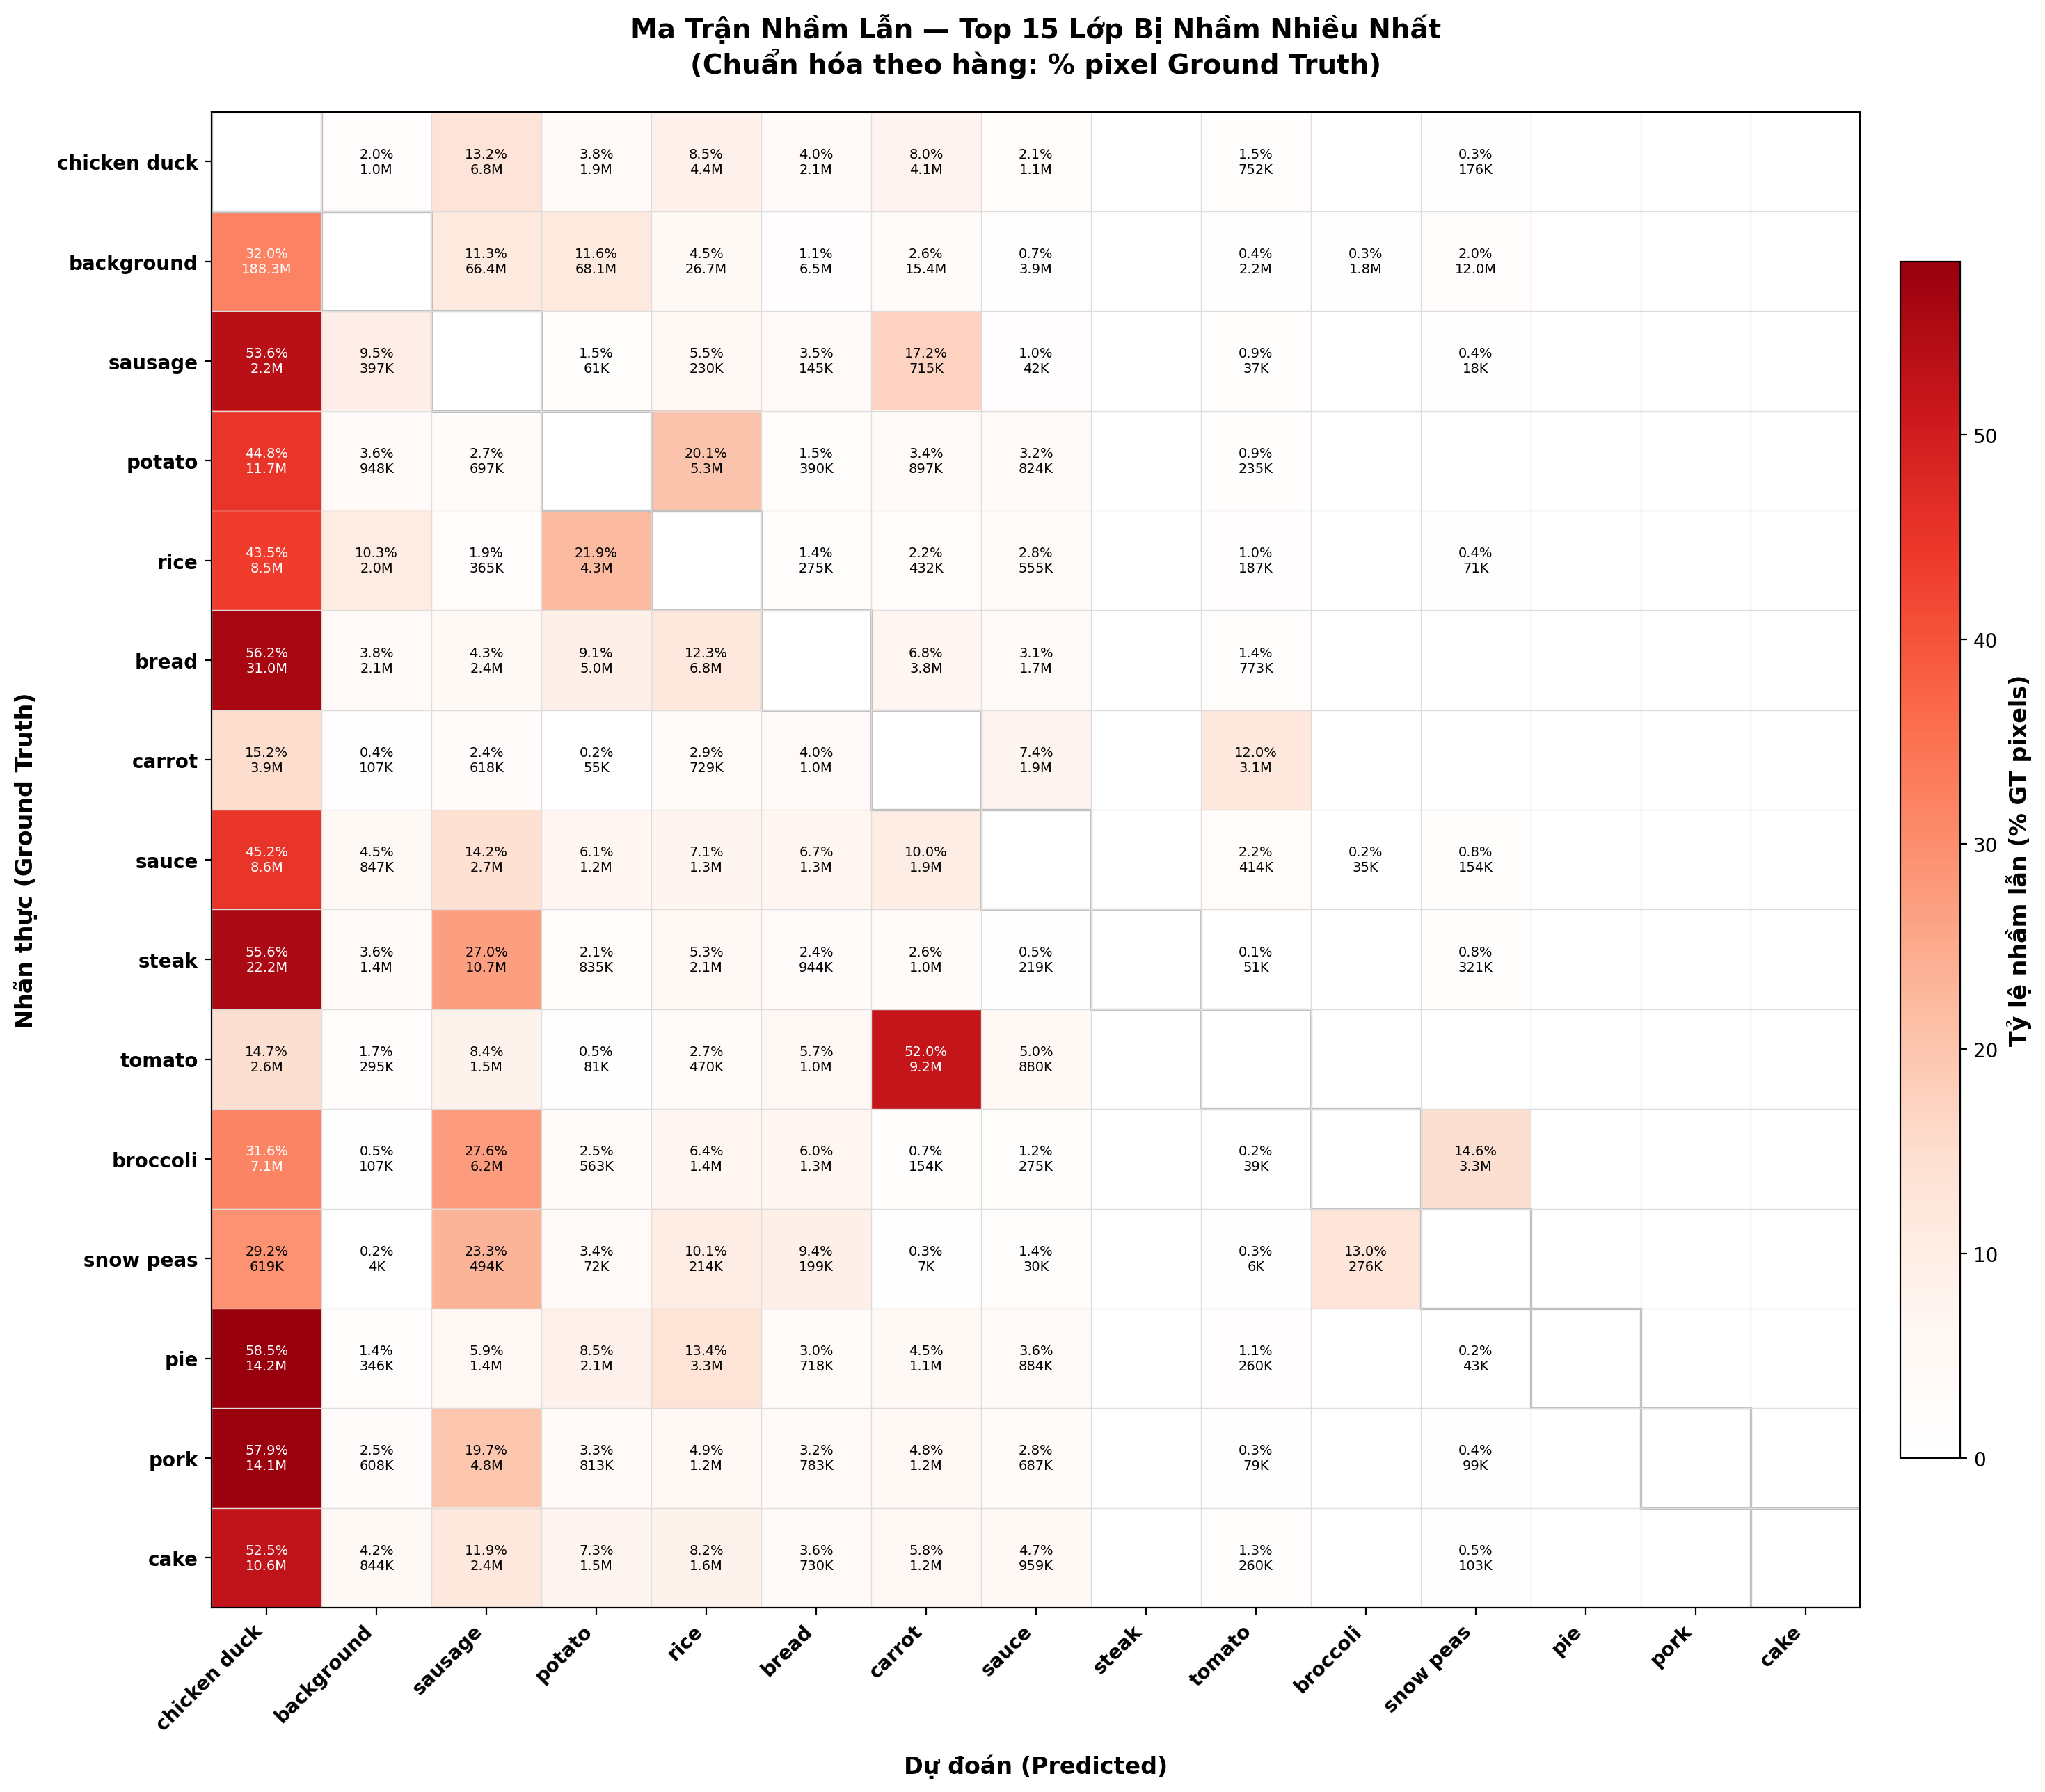
\includegraphics[width=\linewidth]{img/report/analyze/eval-model/04_top_confusion_directions_improved.png}
        \caption{Hướng nhầm lẫn nhiều nhất}
      \end{figure}
  \end{columns}
\end{frame}

\begin{frame}{IV-C. Nhận xét lỗi có cấu trúc}
  \begin{alertblock}{Hiện tượng Sink Class}
    \textbf{chicken duck} thu hút $\approx$458M pixel FP. pie (58.5\%), pork (57.9\%), bread (56.2\%), steak (55.6\%) đều bị kéo về lớp này
  \end{alertblock}
  \vspace{0.3em}
  \textbf{Nhầm lẫn có ý nghĩa thị giác}
  \begin{itemize}
    \item rice $\leftrightarrow$ potato (21.9\% / 20.1\%)
    \item steak $\to$ sausage (27.0\%), broccoli $\to$ sausage (27.6\%)
  \end{itemize}
  \vspace{0.3em}
  \begin{block}{Kết luận}
    Lỗi \textbf{không ngẫu nhiên}: do tương đồng texture + quan hệ đồng xuất hiện. Spatial Path chưa đủ để phân biệt fine-grained texture.
  \end{block}
\end{frame}
